% -*- coding: utf-8 -*-
%%
%%
%%
%%
%%
%%
%%  本模板可以使用以下两种方式编译:
%%
%%     1. PDFLaTeX
%%
%%     2. XeLaTeX [推荐]
%%
%%  注意:
%%    1. 在改变编译方式前应先删除 *.toc 和 *.aux 文件,
%%       因为不同编译方式产生的辅助文件格式可能并不相同。
%%
%%
\documentclass[12pt,openright,openany]{book}


\usepackage{ifxetex}
\ifxetex
  \usepackage[bookmarksnumbered]{hyperref}
\else
  \usepackage[unicode,bookmarksnumbered]{hyperref}
\fi

\usepackage[emptydoublepage]{NKThesis}   % 中文
%\usepackage[emptydoublepage,English]{NKThesis} % 英文

\usepackage{listings}
\usepackage{color}
\usepackage{xcolor}

\usepackage{amsmath}
\usepackage{bm}
\usepackage{amssymb}
\usepackage[ruled,vlined,algochapter]{algorithm2e}
\usepackage{subfigure}
\usepackage{multirow}
\usepackage{float}
\usepackage{booktabs}
\usepackage{fix-cm}

%   根据需要选择 biblatex 宏包选项.
%\usepackage[backend = biber, defernumbers = true,  sorting=none,  style = nkthesis]{biblatex}
%  https://github.com/hushidong/biblatex-gb7714-2015
%  gbpub选项用于处理当出版商、会议地址等不存在时处理
%  gbpunctin选项用于处理连续出版物如会议等时,处理符号"//",这是默认输出,当前为in:
%  gbnamefmt选项默认情况下gbnamefmt=uppercase,作者姓名字母全部大写;
%              当设置gbnamefmt=lowercase时,biblatex-gb7714-2015宏包对于bib文件中的作者姓名的大小写不做改变。
\usepackage[backend=biber,style=gb7714-2015,gbpunctin=false,gbpub=false,gbnamefmt=lowercase]{biblatex}

% hyperref宏包设置命令,下面的组合可以让正文和参考文献中的链接都显示为黑色
\hypersetup{colorlinks=true,
            pdfborder=0 0 1,
            urlcolor=black,
            citecolor=black,
            linkcolor=black}

\raggedbottom

\addbibresource{nkthesis.bib}
\DeclareBibliographyCategory{cited}
\AtEveryCitekey{\addtocategory{cited}{\thefield{entrykey}}}

\includeonly{
abstract,
manual,
references,
acknowledgements,
resume
}
\newtheorem{Theorem}{\hskip 2em 定理}[chapter]
\newtheorem{Lemma}[Theorem]{\hskip 2em 引理}
\newtheorem{Corollary}[Theorem]{\hskip 2em 推论}
\newtheorem{Proposition}[Theorem]{\hskip 2em 命题}
\newtheorem{Definition}[Theorem]{\hskip 2em 定义}
\newtheorem{Example}[Theorem]{\hskip 2em 例}

\renewcommand\listfigurename{图清单}
\renewcommand\listtablename{表清单}
\renewcommand{\algorithmcfname}{算法}
\renewcommand\appendixname{ }

\hyphenpenalty=5000
\tolerance=1000

\newlength{\largNum}

\newlength{\tocRightMargin}
\setlength{\tocRightMargin}{2cm}

\newlength{\tocLeftMarginSecondLineFigure}
\setlength{\tocLeftMarginSecondLineFigure}{6.5em}

\makeatletter
\renewcommand*\l@figure[2]{%
  \settowidth{\largNum}{\hss #2}
  \ifnum \c@tocdepth >\m@ne%
    \addpenalty{-\@highpenalty}%
    \vskip 1.0em \@plus\p@%
    \setlength\@tempdima{3.4em}%
        \noindent%
    \begingroup
      \pretolerance=10000
      \parindent \z@ \rightskip \tocRightMargin%
      \parfillskip -\tocRightMargin%
     \leavevmode \normalsize%
     \advance\leftskip \tocLeftMarginSecondLineFigure%
      \hskip -\leftskip%
      {\figurename\mbox{\hspace{4pt}}#1}\nobreak%
       \leaders\hbox{$\m@th%
        \mkern \@dotsep mu\hbox{.}\mkern \@dotsep%
        mu$} \hfil\nobreak\hb@xt@%
                    \largNum{\hss #2}\par%
      \penalty\@highpenalty%
    \endgroup
  \fi}
\makeatother

\makeatletter
\renewcommand*\l@table[2]{%
  \settowidth{\largNum}{\hss #2}
  \ifnum \c@tocdepth >\m@ne%
    \addpenalty{-\@highpenalty}%
    \vskip 1.0em \@plus\p@%
    \setlength\@tempdima{3.4em}%
        \noindent%
    \begingroup
      \pretolerance=10000
      \parindent \z@ \rightskip \tocRightMargin%
      \parfillskip -\tocRightMargin%
     \leavevmode \normalsize%
     \advance\leftskip \tocLeftMarginSecondLineFigure%
      \hskip -\leftskip%
      {\tablename\mbox{\hspace{4pt}}#1}\nobreak%
       \leaders\hbox{$\m@th%
        \mkern \@dotsep mu\hbox{.}\mkern \@dotsep%
        mu$} \hfil\nobreak\hb@xt@%
                    \largNum{\hss #2}\par%
      \penalty\@highpenalty%
    \endgroup
  \fi}
\makeatother



\begin{document}

%  设置基本信息
%  注意:  逗号`,'是项目分隔符. 如果某一项的值出现逗号, 应放在花括号内, 如 {,}
%
\NKTsetup{%
  论文题目(中文) = 面向室内结构化和开放空间中智能终端用户定位的部分关键技术研究,
  副标题         = ,
  论文题目(英文) = Research on Smart Terminal Users Positioning in Indoor Structured and Open Space,
  论文作者       = 于文平,
  学号           = 1120140111,
  指导教师       = {张建忠\quad 教授},
  申请学位       = 博士,
  培养单位       = 网络空间安全学院,
  学科专业       = 计算机科学与技术,
  研究方向       = 移动计算,
  答辩委员会主席 = 李文龙,
  论文评阅人 = {张老师,徐老师},
  中图分类号     = ,
  UDC            = ,
  学校代码       = 10055,
  密级           = 公开,
                   % 公开 | 限制 | 秘密 | 机密, 若为公开, 不填以下三项
  保密期限       = ,
  审批表编号     = ,
  批准日期       = ,
  论文完成时间   = 二〇一八年十月,
  答辩日期       = ,
  论文类别       = 博士,
                   % 博士 | 学历硕士 | 专业学位硕士 | 同等学力硕士
  院/系/所       = ,
  专业           = ,
  联系电话       = ,
  Email         = yuwenping@mail.nankai.edu.cn,
  通讯地址(邮编) = ,
  备注           = ,
  是否批准为非公开论文 =,}

% -*- coding: utf-8 -*-

%\clearpage
%\addcontentsline{toc}{chapter}{摘要}
\begin{zhaiyao}
随着互联网技术的快速发展,移动设备迅速普及,移动应用数量也呈现爆炸式增长。这些新应用在给用户带来方便的同时,也使得移动网络管理面临更大的挑战。
\\
\end{zhaiyao}

\begin{flushleft}
\begin{guanjianci}
移动应用;卷积神经网络
\end{guanjianci}
\end{flushleft}

%\clearpage
%\addcontentsline{toc}{chapter}{Abstract}
\begin{abstract}
The number of mobile applications is growing explosively, due to the rapid development of the Internet and the widespread of the mobile device. The new applications bring not only the convenience, but also the difficulty to network management. 
\\
\end{abstract}

\begin{flushleft}
\begin{keywords}
mobile application; convolutional neural network
\end{keywords}
\end{flushleft}

\tableofcontents
\listoffigures
\listoftables
% -*- coding: utf-8 -*-


%%------------------------------------------------Chapter Separator-----------------------------------------------%%


\chapter{绪论}

\section{研究背景与意义}

这里来说明室内定位的研究与意义,随着物联网的快速发展,各种应用对于室内定位的需求也与日俱增,这里是测试正文中的链接的\url{https://www.baidu.com/},期望显示的不是红色。

随着无线通信、计算机和感知技术的发展,普适计算实现了物理世界和信息空间的融合,为人们提供了越来越广泛的计算和服务。普适计算中的位置感知计算变得尤为重要,因为多数服务都依赖于位置服务,而随着智能移动设备的普及,基于位置感知计算的服务也变得多种多样。目前,LBS已经成为非常有前景的研究热点之一。它能广泛支持需要动态位置信息的应用,为诸如交通导航、生活信息查询、医疗救护等提供较为准确的位置信息,因此为用户提供LBS有着巨大的市场规模和良好的商业前景。

在开阔的室外环境中,定位和导航服务主要利用全球导航卫星系统(Global Navigation Satellite System, GNSS),主要包括美国的全球定位系统(Global Positioning System, GPS)、俄罗斯的格洛纳斯系统(GLONASS)、欧洲的伽利略系统(Galileo)和中国的北斗卫星导航系统。其中,美国的GPS系统是应用最为广泛且发展较成熟的定位系统,其中民用GPS定位系统的精度可达10米左右,并且最新的GPS系统,通过地面站的位置校准等增强技术,其定位精度可以提高至2~3米左右,能够满足大多数室外LBS服务对于位置信息的精度要求。

但是,上述定位系统都不能用于室内环境下位置感知应用。由于建筑物外墙等对于卫星和基站信号的遮挡,以及复杂的室内环境带来的无线信号传播的多径效应的影响,原有技术手段和算法难以实现在室内环境下的高精度定位。与室外环境相比,室内环境更加复杂,存在着不同类型的干扰源。例如,室内建筑结构和家具等对于电磁波的传播路径的影响从而导致多径效应,来自其他无线设备的干扰和噪声等。所以,开发一种定位精度高、实时性好、经济成本低、可扩展性高的定位技术成为各大互联网企业和研究机构关注的热点课题。到目前为止,研究人员已经将多种技术和方法应用于不同场景下的室内定位系统中,其中,技术手段主要包括红外线、超声波、无线电射频识别(Radio Frequency Identification, RFID)、蓝牙、超宽带(Ultra-wide band, UWB)、地磁场以及无线局域网(802.11, Wi-Fi)等。



\section{室内定位技术分类}

这里想通过室内定位技术的分类来引出指纹定位和行人航位推算技术的详细介绍。

典型的Wi-Fi位置指纹定位算法大体上可以分为两类,即基于近邻选择和基于机器学习的算法。基于近邻选择的算法主要有NN、kNN和w-kNN。近邻选择算法将在线采集到的RSS作为特征值,将其和离线阶段获得的指纹数据库中的RSS样本进行匹配并选择其中最相似的一个或者k个参考点,通过平均或者加权平均k个参考点的位置坐标作为定位结果。基于机器学习的位置指纹定位算法利用离线采集的RSS样本训练确定性或者概率性数学模型,进行确定模型参数,得到一个RSS样本作为输入、位置坐标作为输出的映射关系。在在线阶段,将在线RSS作为模型输入,计算得出定位结果。基于机器学习的位置指纹定位算法有ANN和SVR等。由于RSS的动态变化,典型的Wi-Fi位置指纹定位算法存在着定位结果稳定性比较差的问题。如图XX所示,在同一位置来自同一个无线热点(AP)的RSS的变化情况。

\subsection{行人航位推算}
这里详细说明行人航位推算的原理,以及简单的说明行人航位推算技术的优缺点




\section{结构化空间和开放空间的定义}

这一小节的位置还有待后续斟酌,当前先放在这里吧。

这里给出关于结构化空间和开放空间的抽象定义,用于后续讨论的基础,这里最好给出一个相对详细且抽象的定义,因为这两个概念的定义是后续讨论的基础,所以这里的定义最好能够给人以信服,且最好能够通过引用权威论文来加强说服力,在这一方面,当前还是存在着一定的困难。

\section{国内外研究现状}

国内外研究现状需要从室内定位中与本文相关的部分来进行总结,并且需要设计到较多的参考文献,并且这里的行文的说法也很重要,国内外研究现状的篇幅大概在2-3页。

\section{论文章节安排}

本论文面向室内结构化空间和开放空间的行人定位问题,分析不同室内环境和应用场景下对于室内行人定位方法在部署成本、可扩展性,定位能耗以及定位精度和稳定性等方面的不同需求。本论文共分七章,图x展示了包含本章在内的各章逻辑关系。本文的主要工作应该包括全文的一个整理思路,后续章节中隐含的逻辑关系也应该从这里得到清晰的了解,并且最好通过一个简单清晰的图来说明。


%%------------------------------------------------Chapter Separator-----------------------------------------------%%


\chapter{行人定位算法概述}

\section{典型的Wi-Fi定位算法}

这里介绍典型的Wi-Fi定位算法,例如kNN、Bayes和SVR等。

\section{行人航位推算原理}

这里介绍行人航位推算的原理,行人航位推算的原理图可以放到这里来。

\begin{figure}[htb]
	\centering
	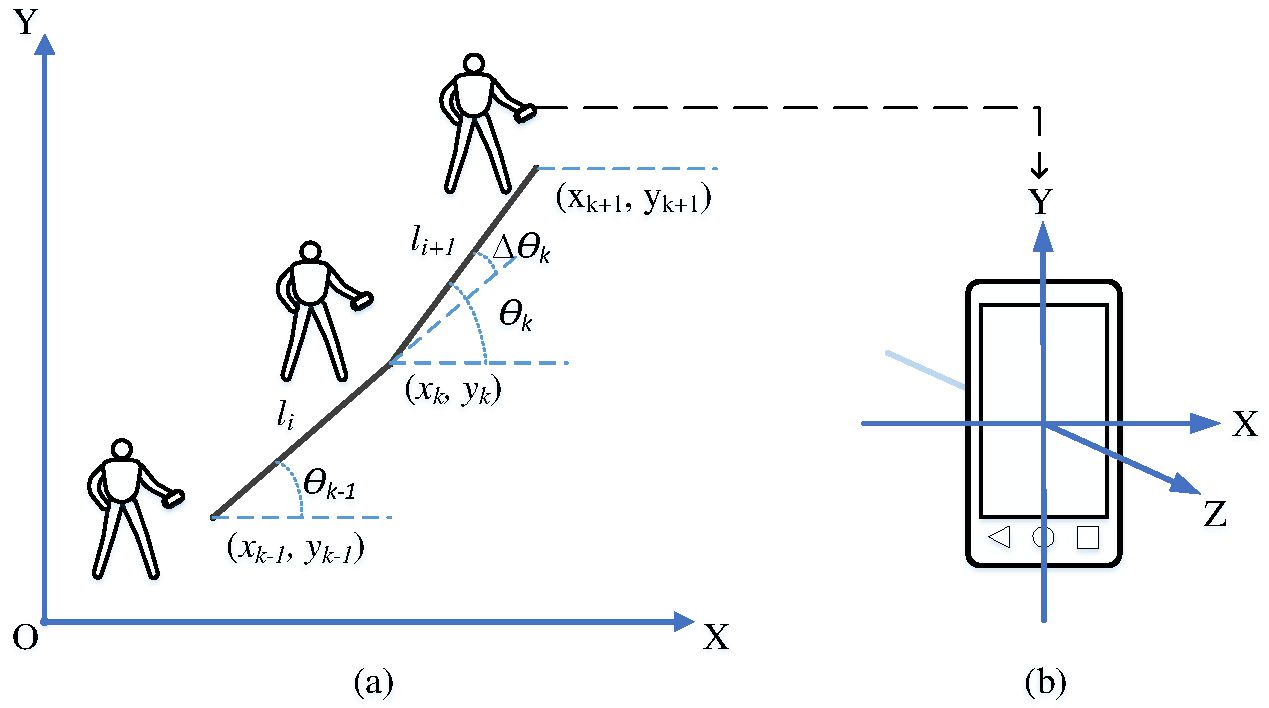
\includegraphics[width=4.75in]{./figures/2/IndoorPos-PDRSchema}
	\caption{行人航位推算原理示意图 (a)全局坐标系下行人航位推算;(b)设备坐标系。}
	\label{fig-pdr}
\end{figure}

\section{主要的滤波算法}

这里介绍卡尔曼滤波和粒子滤波的算法的数学模型和适用情况。

\section{实验环境}

这里主要描述用于后续文章实验的实验场景,其中主要包括实验环境,智能移动设备和参试人员的介绍等。

\section{本章小结}

在这里主要是总结这一章节的内容,如果必要,可以特别简单的引出下一章节的内容。


%%------------------------------------------------Chapter Separator-----------------------------------------------%%


\chapter{面向大规模结构化空间中的行人自主定位}

\section{引言}

在引言中必须说明该章节想要解决的主要问题,并且对问题进行一个简要清晰的描述,一便于后续的理解。

室内定位技术多种多样,但是在实际应用中还存在着许多问题,本章主要从成本和安全两个方面来考量。

\section{模型建立}

模型建立小节主要来详细说明算法的设计细节。

\section{实验分析}

\subsection{实验设置}
通过实验来对算法中的参数或者目标进行对比分析。
\subsection{性能分析}

\section{本章小节}

针对引言中所给出的问题,总结本章。


%%------------------------------------------------Chapter Separator-----------------------------------------------%%


\chapter{从结构化空间到开发空间:基于群智感知的行人定位}

\section{引言}

在引言中必须说明该章节想要解决的主要问题,并且对问题进行一个简要清晰的描述,一便于后续的理解。

考虑到公共空间,如商场、体育馆、火车站、地铁站等,其室内建筑结构不仅包含结构化空间,还包含开发空间,而从结构化空间进入开放空间以后,由于缺少地标点,进而基于PDR技术的行人定位的实现存在着较大的困难,本章中讨论通过基于众源的AP热点位置估计算法来实现行人从结构化空间到开放空间的无缝定位。

\section{模型建立}

模型建立小节主要来详细说明算法的设计细节。

\section{实验分析}

\subsection{实验设置}
通过实验来对算法中的参数或者目标进行对比分析。

\subsection{性能分析}

\section{本章小节}

针对引言中所给出的问题,总结本章。


%%------------------------------------------------Chapter Separator-----------------------------------------------%%


\chapter{基于众源生成的Wi-Fi指纹库的定位技术研究与分析}

\section{引言}

在引言中必须说明该章节想要解决的主要问题,并且对问题进行一个简要清晰的描述,一便于后续的理解\cite{montoliu2017indoorloc}。

基于众源生成的Wi-Fi指纹库由于指纹生成方式的不同,相比于通过专业人士现场测量而得到的Wi-Fi指纹库,存在着两个主要的不同点,一个是由于上传指纹位置的随机性而导致的指纹数据覆盖范围的不平衡性;一个是由于上传指纹的设备的多样性而导致的指纹数据的不一致性。

\section{模型建立}

模型建立小节主要来详细说明算法的设计细节。

\subsection{精度自定义}



\section{实验分析}

\subsection{实验设置}
通过实验来对算法中的参数或者目标进行对比分析。

\subsection{性能分析}

\section{本章小节}

针对引言中所给出的问题,总结本章。


%%------------------------------------------------Chapter Separator-----------------------------------------------%%


\chapter{人机混合场景:基于智能移动机器人辅助的行人定位}

\section{引言}
随着传感器技术、机器人技术以及人工智能技术的发展,智能移动终端越来越多的融入到工业生产、智能仓库、会展导航和家庭清洁等日常生产和生活的许多方面,并且在可预期的将来,智能移动机器人的应用场景日趋丰富,并且成为人们不可或缺的伙伴和帮手。

\section{Android平台简介}

在智能手机领域,Android操作系统自从上市以来,凭借其良好的运行性能和方便的开发环境迅速占领了智能手机市场,如表\ref{tab-61}所示,根据市场调研机构Gartner在2018年2月份发布了一份报告显示2017年全年Android手机市占率高达85.9\%\cite{gartner-smartphone-2017}。


\begin{table} [thb]
	\caption{2017年全球智能手机销售给最终用户统计}\label{tab-61}
	\small
	\centering
	%[t]
	{
		\begin{tabular}{c c c c c}
			\toprule
			操作系统 & 2017(千部) & 2017市场占有率(\%) & 2016(千部) & 2016市场占有率(\%)\\
			\midrule
			Android & 1320118.1 & 85.9 & 1268562.7 & 84.8\\
			iOS & 214924.4 & 14.0 & 216064.0 & 14.4\\
			其他 & 1493.0 & 0.1 & 11332.2 & 0.8\\
			总计 & 1536535.5 & 100.0 & 1495959.0 & 100.0\\			
			\bottomrule
		\end{tabular}
	}
\end{table}


\section{定位技术实现}

在本小节中给出基于Android平台实现过程中遇到的问题,比如设计到众源算法时需要提高算法的处理时间等。

\section{公开数据集的建立}

通过多个Android手机平台上运行定位APP,进而建立公开的数据集方便后续其他定位技术的研究人员来进行定位算法的对比实验研究。


%%------------------------------------------------Chapter Separator-----------------------------------------------%%


\chapter{总结与展望}

\section{本文总结}

现在的定位算法没有考虑手机不同的携带位置对于定位结果的影响。

随着物联网技术的发展和智能移动设备的普及,特别是未来可穿戴设备如智能手环、智能手表、智能眼镜的流行,基于位置的服务在日常出行、医疗监护、应急救援、智能广告等各种方面展示了良好体验和应用前景,因此越来越受到人们的关注和重视。近年来,由于WLAN已经广泛布置于室内环境,基于Wi-Fi的位置指纹定位技术倍受人们的青睐并成为当前国内外的研究热点。本文在对Wi-Fi位置指纹定位各个关键环节深入研究的基础上,以通过众源的方式提高位置指纹数据库的构建效率、定位算法的可扩展性。

\section{后续工作安排}

总结本文,并给出后续的工作安排。

本文的定位技术主要面向室内二维平面的定位,虽然在引入楼层的信息后,上述定位技术很容易扩展至整栋建筑的室内定位,但是上述定位技术并不能给出定位目标的高度信息。

本文给出的定位技术的定位精度都在1~3米级别,面对物联网应用中对于室内高精度的定位需求,本文讨论的算法在定位精度上还不能满足

在现有研究基础上,未来将继续对组合定位算法进行优化,以提高算法的定位精度、可扩展性和可靠性。同时,未来将针对更多的运动模式和导航场景进行研究,以提高算法适用性,将定位算法扩展到更多应用领域,如智能手表、智能眼镜等可穿戴设备上。更进一步挖掘用户导航数据,提高众源数据库的质量和效率。具体可以从以下几个方面进行研究:

\begin{enumerate}[1{)}]
	\item 考虑将基于遗传算法的路径规划算法运用在地磁匹配算法中进一步提高指纹匹配算法的使用效率;
	\item 结合地图匹配技术,利用地图信息进一步提高定位可靠性和定位精度。
	\item 目前组合定位算法针对的行人日常行走的模式,未来针对人在汽车、骑车、跑步等更多运动模式进行进一步的研究,扩展算法的应用领域;
	\item 室内外低能耗的无缝定位是未来的发展趋势,因此定位系统需要考虑将室内和室外定位信息融合,以实现无处不在的定位服务;
	\item 个人隐私和保护越来越受到人们的重视,因此未来的定位系统特别需要考虑在定位过程中对于被服务者的个人隐私的保护的研究。
\end{enumerate}

%%------------------------------------------------Chapter Separator-----------------------------------------------%%


\chapter{南开大学学位论文格式宏包 NKThesis 使用说明} \label{chpt:A}

\section{系统要求}

模板仅在 TeXLive 2016 下测试通过。对于其它 TeX 发行版可能需要做个别修改。


\section{NKThesis 使用说明}

本模板可以使用以下两种方式编译:
\begin{enumerate}
 \item PDF\LaTeX

 \item \XeLaTeX [推荐]
\end{enumerate}

例如,
\begin{verbatim}
         pdflatex main
         bibtex main     % 处理参考文献
         pdflatex main   % 连续编译两遍
         pdflatex main   % 以生成正确的文献引用。
\end{verbatim}

本模板用到 宋体、楷体、仿宋、黑体四种字体\cite{GB25100—2010}. 若需重新配置字体, 请修改 NKTfonts.cfg.
对于 Linux/Mac 下的 TeX Live 2009, 可能需要设置环境变量 OSFONTDIR, 具体内容请参考 texmf.cnf.

我们建议您使用\XeLaTeX\ 编译。与前两种方法相比,\XeLaTeX\  编译长文档的速度更快,
编译一篇一百多页的论文只需几秒的时间(SL9400 @ 1.86GHz)。

在改变编译方式前应先删除 *.toc 和 *.aux 文件,
因为不同编译方式产生的辅助文件格式可能并不相同。

注意:使用 \XeLaTeX\ 编译时,\XeTeX\ 的版本应不低于 0.9995.0(MiKTeX 2.8 或者 TeXLive 2009)。


\section{引用章节号}
\label{sec:ex:A}

引用章节号请参考如下格式: \ref{chpt:A}\ref{sec:ex:A}.


\section{中英文间隔}

使用 \XeLaTeX\ 编译时,会自动在中英文转换时添加必要的空格。 使用 [PDF]\LaTeX\
编译时仅忽略中文之间的空格,而中英文之间的空格予以保留。
因此,不管何种编译方式,您都不需要在中英文间添加 $\tilde{}$ 以获得额外的空格。例如,

这是 English 中文 $x=y$ 测试

这是English中文$x=y$测试

可以看出,以上两行用 \XeLaTeX\ 编译的结果是相同的。


%%------------------------------------------------Chapter Separator-----------------------------------------------%%


\chapter{引言}

\section{研究背景}

随着计算机技术和互联网技术的快速发展\cite{Nadkarni-1992},各式各样的网络应用伴随着人们的需求应运而生\cite{Hua-Wang-1973}。

\subsection{研究意义}

随着计算机技术和互联网技术的快速发展\cite{Nadkarni-1992},各式各样的网络应用伴随着人们的需求应运而生\cite{Hua-Wang-1973}。

\begin{table} [thb]
	\caption{常见端口协议映射表}\label{tab:21}
	\small
	\centering
	%[t]
	{
		\begin{tabular}{cccc}
			\toprule
			Port & Protocol & Port & Protocol\\
			\midrule
			21 & FTP & 88 & Kerberos\\
			22 & SSH & 109 & POP\\
			23 & Telnet & 110 & POP3\\
			25 & SMTP & 115 & SFTP\\
			37 & TIME & 143 & IMAP4\\
			43 & WHOIS & 161 & SNMP\\
			53 & DNS & 179 & BGP\\
			80 & HTTP & 443 & HTTPS\\
			
			\bottomrule
		\end{tabular}
	}
\end{table}

网络流量的不断增长给网络管理带来了巨大难题。

\begin{figure}[htb]
\centering

\includegraphics[width=3.8in]{./figures/0/nankaidaxue}
\caption{南开大学标准图片}
\label{fig:11}
\end{figure}

近几年来,随着手机、平板电脑、智能手环等移动设备的普及\supercite{bahl2000radar},移动互联网用户不断增多\supercite{monkey}。
%% -*- coding: utf-8 -*-

% -*- coding: utf-8 -*-

%\def\bibrangedash{ $\sim$ }
\renewcommand*{\bibfont}{\small}
\nocite{*}
%\printbibliography[category = cited]
\printbibliography[title=参考文献]
%\printbibliography[heading=bibliography,title=参考文献]

%\def\bibrangedash{ $\sim$ }
%\printbibliography [ category = cited]
% -*- coding: utf-8 -*-

%\makeschapterhead{致谢}
\chapter*{致谢}

{\fangsong 依稀记得2014年初秋博士入学时自己难以掩饰的喜悦之情以及对未来的企盼,新开湖畔的背影脚步匆匆,马蹄湖上的荷花谢了又开,转眼已是将近五年,这期间,有过明日复明日的拖沓与懒惰,亦有过只争朝夕的坚持与奋发。值此博士论文完稿之际,谨对给予我帮助和支持的老师、同学和家人致以衷心的感谢。}

{\fangsong 首先,感谢我的导师张建忠教授,本文的研究工作是在张老师的悉心指导下完成的,从论文选题、资料查找、开题报告、研究思路和成果总结等各个方面,张老师都给予了我许多宝贵的意见。张老师,谆谆教诲,亦师亦长,在攻读博士学位期间,无论在治学还是在为人上都让我受益良多。}

{\fangsong 其次,感谢徐敬东教授,徐老师精深的专业知识和认真的科研作风一直影响着实验室的每一位学生。感谢吴英副教授,吴老师工作上一丝不苟,生活中平易随和,是一位值得信赖的老师。感谢张玉副教授,张老师旺盛的科研热情让人敬佩,在张老师的带领下,得以参与许多国家重大科研项目的申请和研究,极大地拓宽了我的学术视野。}

{\fangsong 特别感谢许昱玮副教授和蒲凌君老师,两位年轻老师都面临着极大的学术压力,但仍不厌其烦,或帮我思考科研规划,或帮我理清研究思路,或帮我修改学术论文,在生活和科研上为我提供了许多无私的帮助。}

{\fangsong 感谢林进挚、林安华、王昌海、于博文师兄,感谢实验室已经毕业和尚未毕业的师弟师妹们,独学而无友,则孤陋而寡闻,在求学的路上同你们一起前行,幸甚至哉。}

{\fangsong 最后,必须要感谢的是我的家人,是你们包容、鼓励和支持,才让我坚持至今。感谢我的父亲和母亲,二老都已过耳顺之年,白发渐多,皱纹日深,作为儿子不能尽孝于膝前,心中多有愧疚,谨以此文献给你们,祝愿二老身体健康。感谢我的姐姐和姐夫,从我博士入学的那日起,你们不仅担负了照顾父母的重任,还时时敦促我的学业,祝你们家庭和美,事事顺心。感谢我的女朋友,平平淡淡中已经陪我走过多年,愿与你一直走到天涯海角。}

% -*- coding: utf-8 -*-


\chapter*{个人简历、在学期间发表的学术论文与研究成果}
\section*{个人简历}
于文平,男,1986年02月01日出生。2004年9月至2008年6月就读于南开大学信息技术与科学学院计算机科学与技术专业,获工学学士学位;2008年9月至2011年6月就读于南开大学信息技术与科学学院学院计算机科学与技术专业,获工学硕士学位;2014年9月至2019年6月就读于南开大学计算机与控制工程学院(现改为网络空间安全学院)计算机科学与技术专业,攻读博士学位,研究方向为室内定位。
\section*{发表论文}
\begin{enumerate}
\renewcommand{\labelenumi}{[\theenumi]}
\item Yu Wenping, Zhang Jianzhong, Xu Jingdong and Xu Yuwei. Motion Trajectory Sequence-Based Map Matching Assisted Indoor Autonomous Mobile Robot Positioning[C]. ICA3PP. Springer, 2018. (CCF C类,已录用未发表)
\item Yu Wenping, Zhang Jianzhong, Xu Jingdong and Xu Yuwei. An Accurate Indoor Map Matching Algorithm Based on Activity Detection and Crowdsourced Wi-Fi[J]. Sci China Tech Sci. 2018. (SCI 三区,已录用未发表)
\item Yu Wenping, Xu Yuwei, Zhang Jianzhong, et al. A Smartphone-Based Online Pedestrian Positioning Approach for Both Structured and Open Indoor Spaces[C]. ISPA. IEEE, 2017. (CCF C类)
\item Yu Wenping, Zhang Jianzhong and Wang Changhai. An on-demand approach for indoor localization based on crowdsourced Wi-Fi fingerprints[C]. ICCSNT. IEEE, 2015. (EI)
\item Fu Ningjia, Zhang Jianzhong, Yu Wenping and Wang Changhai. Crowdsourcing-based wifi fingerprint update for indoor localization[C]. Proceedings of the ACM Turing 50th Celebration Conference-China. ACM, 2017. (EI)
\end{enumerate}
\section*{参与项目}
\begin{enumerate}
\renewcommand{\labelenumi}{[\theenumi]}
\item 2017年6月 - 至今,基于脑电波的射击校正实验平台
\item 2016年11月 - 2018年5月,非标准和加密VOIP协议的流量识别
\item 2009年9月 - 2011年7月,战地伤员救治卫勤训练系统
\item 2008年11月 - 2009年6月,开放式调度管理系统
\item 2008年7月 - 2008年12月,加密算法生成和校验系统
\end{enumerate}
%\section*{获得奖励}
%2020年xx月xxxx奖学金
\end{document}
